\documentclass[../main.tex]{subfiles}

\begin{document}
    \chapter{Related Work}\label{chap:related}

    \section{Domain Adaptation approaches}\label{sec:related-word}
	Domain Adaptation is a fundamental problem in machine learning, and the need for techniques that works when
	$P_{s}(X, Y) \neq P_{t}(X, Y)$ is preminent in the majority of practical applications. In computer vision in particular,
	there is a large number of factors which can cause the domain shift: background, lighting conditions, resolution and scale,
	position and orientation of the object of interest and so on. Various approaches to address the domain adaptation problem
	have been proposed in the literature. In the following overview of the domain adaptation literature, we will use the same
	distinction of~\cite{DBLP:journals/corr/Csurka17} into shallow methods and the more recent deep methods, which employs
	deep learning models, in particular the deep convolutional networks described in Section~\ref{sec:deeplearning}.

    \subsection{Shallow Methods}
	In this context, shallow methods refers to those methods which are based on feature vector representations $X$ extracted from
	the images with non-deep-learning methods.

	\paragraph{Instance Weighting}
	The earliest solutions to the domain adaptation problem go under the name
	of \textit{Instance Weighting} approaches.
	The basic idea is that of assigning a different weight to each sample in the computation of the loss. The definition of the
	weight varies based on the assumptions one makes about the source and target distributions. One possible approach is assuming
	that the conditional distributions of the labels given the same observation are the same, but clearly the marginal distributions
	of the observations are different. Formally:
	$$ P_{s}(Y | X = x) = P_{t}(Y | X = x) \text{ with } P_{s}(X) \neq P_{t}(X) $$
	This assumption is called \textit{covariate shift} and it is explored in depth in~\cite{shimoidara2000}. To solve the covariate
	shift problem,~\cite{shimoidara2000} weights each training instance with $\frac{P_{t}(X)}{P_{s}(X)}$, that is, the weight is the
	ratio between the likelihood of being a target and a source sample.

	\paragraph{Feature Space Alignment}
	Another class of techniques that tries to align source features with the target ones. A very simple method in this class is
	Subspace Alignment (SA)~\cite{subspace-alignment}, where the alignment is made between the subspaces obtained by PCA reduction:
	$$ P_{s} = PCA(X_{s}, d) \qquad P_{t} = PCA(X_{t}, d) $$
	$$ X_{s}^{'} = X_{s}P_{s}P_{s}^{T}P_{t} \qquad X_{t}^{'} = X_{t} P_{t} $$
	And then $X_{s}^{'}$ and $X_{t}^{'}$ are used in place of $X_{s}$ and $X_{t}$.

	\paragraph{Feature Transformation through metric learning}
	These are semi-supervised domain adaptation methods, as they require at least a limited amount of target labels available.
	One method worth mentioning is DA-NBNN~\cite{da-nbnn}. The main idea of DA-NBNN is to replace at each iteration the most ambiguous
	source example of each class by the target example for which the classifier (Naive Bayes Nearest Neighbor (NBNN)) is the
	most confident for the given class. It does this by iteratively learning a metric of the relatedness between the source and
	target domains.

    \subsection{Deep methods}
	The expression deep methods refers to all those approaches which are based either on fixed features extracted from a deep learning
    model or on the design of a novel deep network architecture which encorporates elements to solve the domain adaptation problem.
    One method worth mentioning in this respect is the Domain Adversarial Neural Networks (DANN)~\cite{DANN}, which obtained state-of-the-art
    results on several benchmark datasets. It is called adversarial training because a part of the network is optimized in such a way
    to confuse another part of the network.

    \subsubsection{DANN}
    Adversarial Training. The networks is composed of three parts:
    \begin{itemize}
        \item \textbf{feature extractor}: this part of the network is trained to simultaneously optimize two objetives: learn features
            that are discriminant for the source classification task, and at the same time learn domain invariant features, that is,
            features that would increase the classification error of a binary domain classifier.
        \item \textbf{image classifier}: this is the classifier that carries on the main image classification task.
        \item \textbf{domain classifier}: this is the binary classifier that carries on the domain classification task between source and
            target. It is the adversary of the feature extractor.
    \end{itemize}

    \begin{figure}
        \centering{}
    	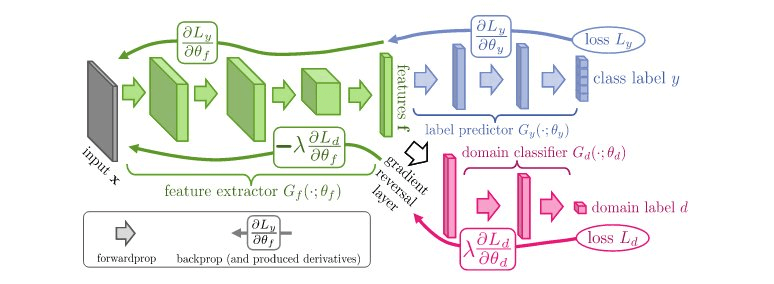
\includegraphics[width=\linewidth]{img/dann-architecture.png}
        \caption{DANN Architecture. Image taken from~\cite{DANN}.}\label{fig:dann-architecture}
	\end{figure}

\end{document}
